\documentclass{beamer}
\usepackage[utf8]{inputenc}
\usepackage[UKenglish]{babel}
\usepackage[UKenglish]{isodate}
\usepackage{tikz}
\usepackage{minibox}

\beamertemplatenavigationsymbolsempty
\usetheme{Madrid}
\usecolortheme{orchid}

\usetikzlibrary{arrows}
\usetikzlibrary{arrows.meta}
\usetikzlibrary{positioning}

\author[P. Dilkas, V. Belle]{Paulius Dilkas \and Vaishak Belle}
\title{WMC with Conditional Weights for BNs}
\date{UAI 2021}
\institute{University of Edinburgh}

\begin{document}

\begin{frame}{Weighted Model Counting with Conditional Weights for Bayesian Networks}
  \begin{columns}
    \begin{column}{0.35\textwidth}
      \centering
      \structure{Probabilistic Inference} \\
      (e.g., a Bayesian network)
      \fbox{
        \begin{minipage}{2.5cm}
          \centering
          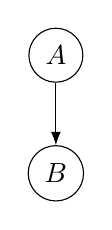
\begin{tikzpicture}[edge from parent/.style={draw,-{Latex}}]
            \node[draw,circle] at (0, 0) (a) {$A$}
            child {node[draw,circle] (b) {$B$}};
          \end{tikzpicture}\\
          Find \alert{$\Pr(B = 0)$}
        \end{minipage}
      }
    \end{column}
    \begin{column}{0.35\textwidth}
      \centering
      \structure{WMC Encoding} \\
      (CNF with literal weights)
      \framebox{
        \scalebox{0.2}{
          \begin{tabular}{@{}l@{}}
            p cnf 8 17 \\
            -2 -1 0 \\
            1 2 0 \\
            -3 1 0 \\
            -1 3 0 \\
            -5 -1 0 \\
            -5 -4 0 \\
            1 4 5 0 \\
            -6 -1 0 \\
            -6 4 0 \\
            -4 1 6 0 \\
            -7 1 0 \\
            -7 -4 0 \\
            -1 4 7 0 \\
            -8 1 0 \\
            -8 4 0 \\
            -4 -1 8 0 \\
            -4 0 \\
            c weights 1.0 1.0 0.5 1.0 0.5 1.0 1.0 1.0 0.6 1.0 0.4 1.0 0.1 1.0 0.9 1.0
          \end{tabular}%
        }
      }

      \vspace{1cm}
      \onslide<2>{
      \structure{Conditional Weights} \\
      \framebox{
        \scalebox{0.2}{%
          \begin{tabular}{@{}l@{}}
            p cnf 2 1 \\
            2 0 \\
            w 1 0.5 0.5 \\
            w 2 1 0.6 0.4 \\
            w 2 -1 0.1 0.9
          \end{tabular}%
        }
      }
      }
    \end{column}
    \begin{column}{0.30\textwidth}
      \centering
      \structure{WMC Algorithm}\\
      \onslide<2>{\alert{$>100\times$} faster}
      % \onslide<2>{\alert{127--$625\times$} faster}
    \end{column}
  \end{columns}
  \begin{tikzpicture}[remember picture,overlay]
    \node at ([yshift=30pt,xshift=-155pt]current page.south)
    {
\includegraphics[height=40pt]{../poster/logo_inf.png}};
    \node at ([yshift=30pt,xshift=-110pt]current page.south)
    {
\includegraphics[height=40pt]{../poster/logo_ecr.png}};
    \node at ([yshift=25pt,xshift=-45pt]current page.south)
    {
\includegraphics[height=20pt]{../poster/logo_ukri.png}};
    \draw[-{Latex}] (3.4, 3) -- (4.9, 4);
    \draw<2>[-{Latex}] (3.4, 3) to [bend right] (5.8, 0.2);
    \draw[-{Latex}] (7.7, 4) -- (9, 2.8);
    \draw<2>[-{Latex}] (6.7, 0.2) to [bend right = 45] (9, 2.8);
  \end{tikzpicture}
\end{frame}
\end{document}